%%%% University of Cambridge tech-report formatting; enable when producing
%%%% tech-report versions of these documents; otherwise, disable.
\documentclass[12pt,twoside,openright,a4paper]{article}
\setlength{\oddsidemargin}{-0.4mm} % 25 mm left margin
\setlength{\evensidemargin}{\oddsidemargin}
\setlength{\textwidth}{160mm}      % 25 mm right margin
\setlength{\topmargin}{-5.4mm}     % 20 mm top margin
\setlength{\headheight}{5mm}
\setlength{\headsep}{5mm}
\setlength{\footskip}{10mm}
\setlength{\textheight}{237mm}     % 20 mm bottom margin
%%%% .. or regular document
%\documentclass[12pt,letterpaper,twoside,openright,fleqn]{report}
%%%% End of tech-report vs. regular
%%%%

\usepackage{graphicx}

\begin{document}

\title{PVMv2 Specification}
\author{Thomas Bytheway & Lucian Carata}

%% CL tech-report format provides its own cover page
\begin{minipage}[h]{\textwidth}
    \maketitle
    \vspace{2in}
    {\small}
\end{minipage}
%%

\normalsize

%% CL tech-report format requires page numbering to start at 3
%\setcounter{page}{3}
%%

%% For revisions sent for editing, prefer double spacing.
%\doublespacing
%%

\clearpage

\section{Introduction}

\section{Types}

\begin{figure}[h]
\centering
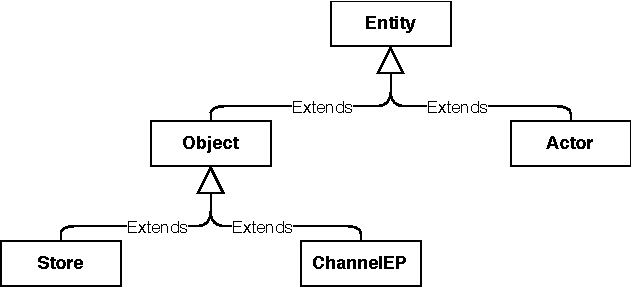
\includegraphics{pvm_types.pdf}
\caption{A diagram of the basic abstract types in PVMv2}
\end{figure}

\paragraph{Entity}

\paragraph{Actor}

\paragraph{Object}

\paragraph{Store}

\paragraph{ChannelEP}

\section{Relations}

\paragraph{INF}

\paragraph{NAMED}

\section{Mappings}

\subsection{Concrete Type Declaration}

\subsection{Verbs}

\paragraph{Declare}

\paragraph{Sink}

\paragraph{Source}

\paragraph{Connect}

\paragraph{Mention}

\paragraph{Unlink}

\paragraph{Property}

\end{document}
